\documentclass[conference]{IEEEtran}

\usepackage{times}
\usepackage{graphicx}
\usepackage{amsmath}
\usepackage{booktabs}
\usepackage{hyperref}
\usepackage{enumitem}
\usepackage{caption}
\usepackage{subcaption}
\usepackage{float}
\setlength{\belowcaptionskip}{-0.2cm}

\begin{document}
\renewcommand{\thesection}{\arabic{section}}
\renewcommand{\thesubsection}{\arabic{section}.\arabic{subsection}}
\renewcommand{\thetable}{\arabic{section}.\arabic{table}}
\renewcommand{\thefigure}{\arabic{section}.\arabic{figure}}


\title{Predicting Novice Programmer Performance from AI-Tutor Interaction Logs Using Machine Learning}

\author{
    \IEEEauthorblockN{Anissa Williams}
    \IEEEauthorblockA{
        MS Data Science \& Analytics \\
        College of Charleston \\
        April 2026
    }
}

\maketitle

\begin{abstract}
This study investigates whether interaction-level behavioral signals from an AI tutoring system can predict student performance in programming tasks. The study was conducted with
second‑semester College of Charleston Computer Science students in Spring
2026. The tutoring system generates rich interaction logs that capture how
students engage with instructional content moment‑to‑moment. This work
uses those logs to investigate whether session‑level behavioral signals—
such as timing, pacing, and interaction volume—can predict student
performance in a programming context. Using 104 complete learning
sessions, we first construct a 16‑feature model incorporating engagement,
temporal, metadata, and difficulty‑weighted features. These models achieve
strong predictive performance (AUC‑ROC up to 0.79), but also exhibit
substantial overfitting, with Random Forest and Gradient Boosting reaching
training accuracies of 0.952 and 1.00, respectively.

Feature analysis reveals that the difficulty‑weighted features introduce
data leakage by partially encoding quiz outcomes. To address this, we
refine the model to a leakage‑free, five‑feature behavioral set. On this
more rigorous formulation, the strongest model (SVM with an RBF kernel)
achieves 0.714 test accuracy, 0.681 cross‑validated accuracy, and a
0.764 AUC‑ROC, demonstrating that behavioral interaction traces alone can
predict performance above chance.


Interpretability analysis using SHAP identifies session duration, response-time pacing, and interaction structure as the most influential predictors. These findings demonstrate the feasibility of real-time, behavior-driven intervention in AI tutoring systems and highlight the importance of rigorous feature design in educational machine learning.

\end{abstract}

\section{Introduction}

Artificial Intelligence in Education (AIED) has increasingly focused on adaptive systems that personalize instruction and provide timely feedback. A central goal in this domain is the early identification of students at risk of poor learning outcomes, enabling intervention \textit{during} the learning process rather than \textit{after} assessment. Predictive modeling plays a key role in this shift from reactive to proactive education.

Recent advances in large language models (LLMs) have introduced conversational AI tutoring systems that interact with students in natural language. These systems generate fine-grained behavioral traces, including timing, pacing, and message exchange patterns, providing a continuous record of student engagement. Prior work in educational data mining shows that behavioral signals correlate with learning outcomes, even in the absence of correctness data \cite{encyclopedia4040108}.

This study investigates whether interaction-level behavioral signals from an AI tutor can predict student performance in a programming context. Using data from a controlled Java tutoring experiment, we analyze session-level interaction logs to evaluate the predictive power of behavioral features.

A key contribution of this work is the identification and correction of a subtle but critical form of data leakage: difficulty-weighted features derived from quiz responses can partially encode the target variable, artificially inflating model performance. By removing these features, we demonstrate that a compact set of behavioral signals alone retains meaningful predictive power.

Unlike many prior studies that rely on observational or platform-aggregated datasets, this work leverages a controlled dataset collected within a university programming course, capturing complete conversational interaction logs between students and an AI tutor. This setting enables fine-grained analysis of behavioral dynamics during learning, providing a level of interaction detail that is not typically available in standard educational datasets.

Specifically, this paper makes four contributions:

\begin{itemize}
    \item Demonstrates that AI tutor interaction logs contain predictive behavioral signals
    \item Identifies and corrects data leakage introduced by quiz-derived features
    \item Shows that behavioral-only models achieve robust performance without reliance on correctness-based inputs
    \item Evaluates these methods on a controlled, conversational dataset collected from a real-world AI tutoring deployment
\end{itemize}



\section{Dataset Description}

\subsection{Source Data}
The dataset consists of 104 completed learning sessions from 52 students enrolled in a second-semester Java programming course. Students interacted with an AI Java tutor across two topics: ArrayLists and Recursion. Each session includes full conversational logs, timestamps, session metadata, and quiz results.

The raw dataset contains approximately 28,600 lines of JSON logs, which were parsed into structured tables representing messages, sessions, and quiz responses. Because the analysis examines behavioral patterns across repeated sessions for each student, only learners who completed both topics were retained. 

\subsection{Target Variable}
Student performance is defined as a binary classification based on quiz scores:
\begin{itemize}[noitemsep]
    \item High performance: $\geq 70\%$
    \item Low performance: $< 70\%$
\end{itemize}


The resulting distribution is approximately balanced 49 High (47.1\%) and 55 Low (52.9\%), supporting reliable model evaluation. 

The mean quiz score across all conditions is 66.9\% and the median is 60\%, reflecting a slight left skew. This distribution was used for all stratified splits and cross‑validation folds.

\subsection{Feature Engineering}
Features were engineered across four categories:
\begin{itemize}
    \item Engagement: total messages, user messages, assistant messages
    \item Temporal: session duration, average response time, response-time variability
    \item Metadata: instructional condition, session type
    \item Difficulty-weighted (later removed): correctness weighted by question difficulty
\end{itemize}

This produced an initial set of 16 features used for exploratory modeling.


\begin{table}[H]
\centering
\caption{Full Feature List}
\begin{tabular}{ll}
\toprule
Feature & Category \\
\midrule
total\_messages & Engagement \\
condition & Metadata \\
session\_type\_enc & Metadata \\
has\_both\_enc & Metadata \\
duration\_seconds & Temporal\\
avg\_response\_time & Temporal \\
min\_response\_time & Temporal \\
std\_response\_time & Temporal \\
median\_response\_time & Temporal \\
assistant\_messages & Engagement \\
user\_messages & Engagement \\
rapid\_response\_pct & Temporal + Engagement \\
rapid\_response\_count & Temporal + Engagement \\

\bottomrule
\end{tabular}
\end{table}


\section{Preprocessing}

The raw dataset consisted of 28{,}600 lines of JSON logs generated by the AI Java Tutor. Each JSON record contained nested structures for messages, timestamps, quiz responses, and metadata. To prepare these logs for modeling, we implemented a multi-stage preprocessing pipeline that transformed the raw JSON into structured, analysis-ready tables.

\begin{figure}[!t]
    \centering
    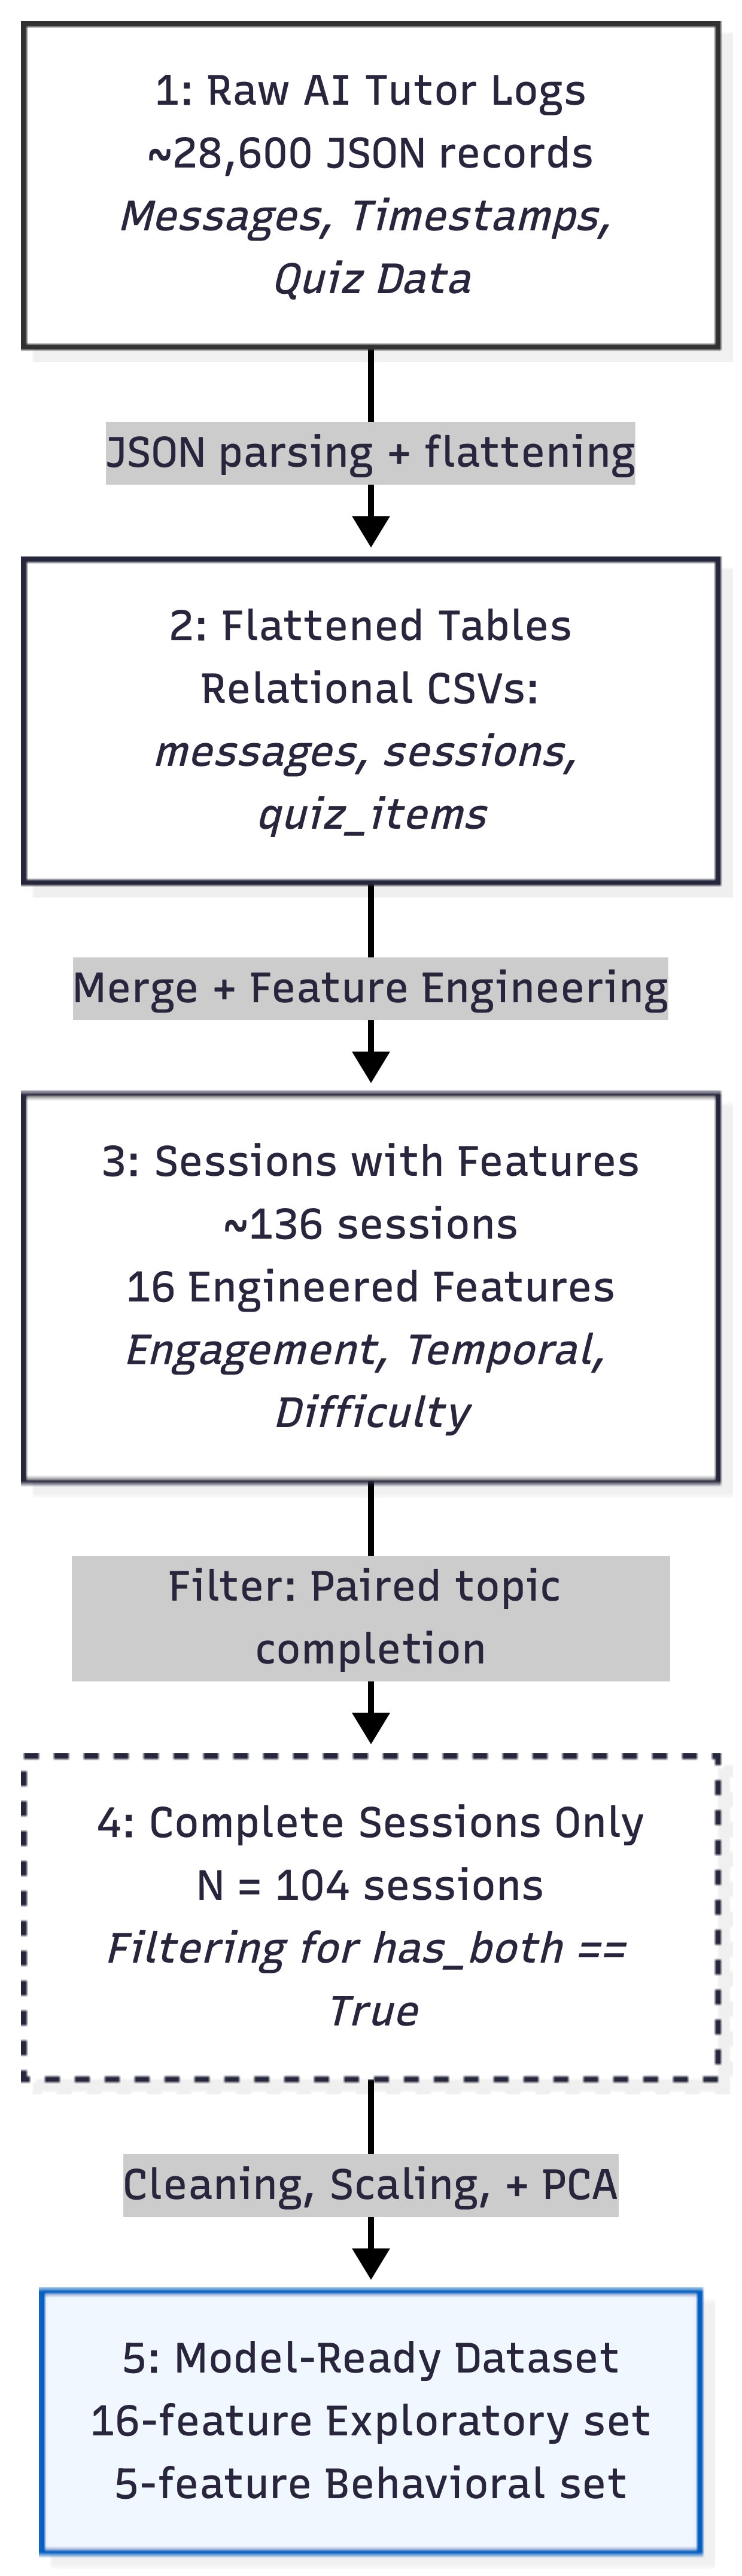
\includegraphics[width=.75\linewidth, height=0.60\textheight, keepaspectratio]{AI Tutor Log Processing-2026-04-23-232835.png}

    \caption{Preprocessing Pipeline}
    \label{fig:placeholder}
\end{figure}

\subsection{JSON Parsing and Flattening}
The first stage involved converting the nested JSON logs into relational tables. Three primary tables were produced:

\begin{itemize}[noitemsep]
    \item \textbf{messages.csv}: one row per message, containing sender (user or assistant), timestamp, and message text.
    \item \textbf{sessions.csv}: one row per session, containing session-level metadata such as topic, instructional condition, and duration.
    \item \textbf{quiz.csv}: one row per quiz item, including correctness and difficulty level.
\end{itemize}

Flattening the logs enabled feature engineering at both the message level (e.g., response times) and the session level (e.g., total messages, duration).

\subsection{Session Merging and Feature Assembly}
The flattened tables were merged into a unified dataset, \textbf{sessions\_with\_engagement\_features.csv}, which contained all engineered features required for modeling. This merge included:

\begin{itemize}[noitemsep]
    \item computing response-time features by differentiating consecutive message timestamps,
    \item aggregating message counts (total, user, assistant),
    \item calculating rapid-response indicators,
    \item attaching quiz-level difficulty information,
    \item creating a boolean feature where the user id for both sessions matched and the sessions were completed
\end{itemize}



\subsection{Filtering for Complete Sessions}
A critical pre-processing step was filtering to sessions where students completed \emph{both} topics (ArrayList and Recursion). This was implemented using the engineered boolean field \texttt{has\_both}.

This step reduced the dataset from about 136 to 104 complete sessions, giving each student a matched pair of sessions and preventing the analysis from being skewed by topic‑specific differences.

\subsection{Cleaning and Imputation}
Several fields required cleaning:

\begin{itemize}[noitemsep]
    \item missing difficulty values were imputed with 0,
    \item response-time nulls were filled with the median response time for that session,
    \item boolean fields were converted to integers,
    \item categorical fields (e.g., session type, instructional condition) were label-encoded.
\end{itemize}

These steps ensured that all features were numeric and compatible with downstream models.

\subsection{Scaling}
All numeric features were standardized using \texttt{StandardScaler}, producing zero-mean, unit-variance inputs. Scaling was particularly important for SVM and PCA, which are sensitive to feature magnitude.


\subsection{Leakage Identification and Feature Refinement}
During feature importance analysis (Fig \ref{fig:importance}), we identified a critical issue: difficulty-weighted features were derived from quiz responses and therefore partially encoded the target variable. This constitutes data leakage, leading to inflated or misguided performance estimates.

To address this, we removed all quiz-derived features. Additionally, the five response-time variants (avg, median, std, min, max) capture highly correlated information, with avg\_response\_time providing the strongest and most interpretable signal. min\_response\_time was the original pacing feature but reflects only a single moment rather than sustained behavioral patterns. It was replaced later by average\_response\_time in the final pipeline.


\begin{figure}[!t]
    \centering
    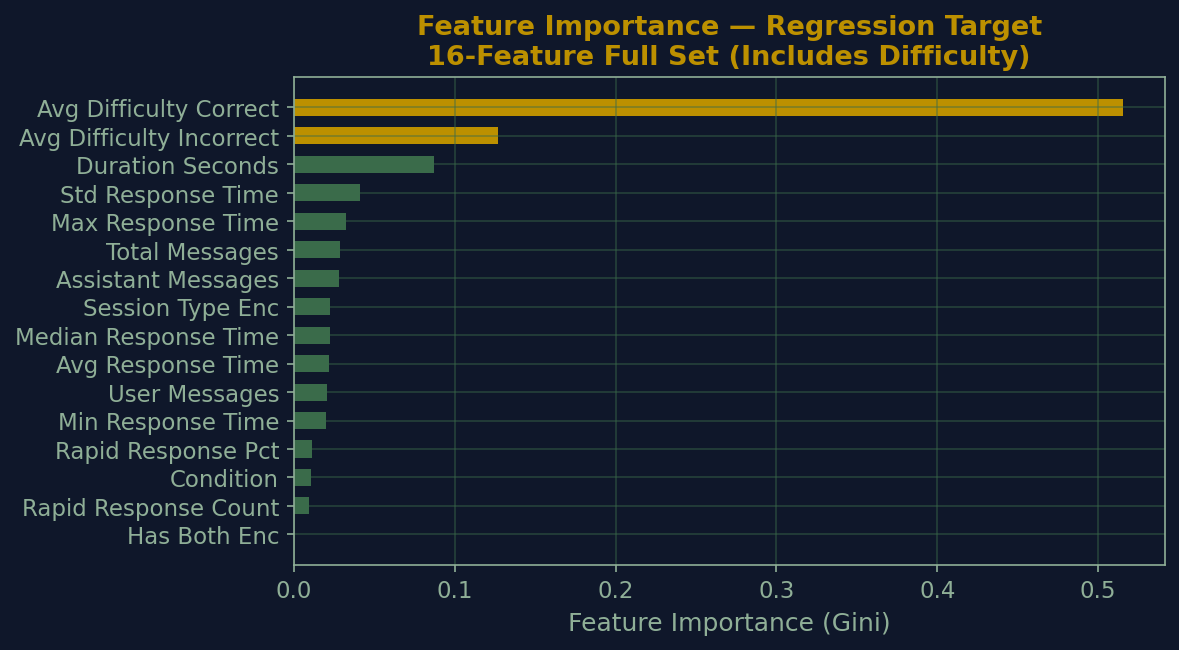
\includegraphics[width=1\linewidth]{16feat_full_feature_importance.png}
    \caption{Feature Importance reveals the quiz-encoded features are highly influential in predictions}
    \label{fig:importance}
\end{figure}


To address the leakage and correlation issues, we refined the dataset to a five-feature behavioral-only model containing no quiz-derived information: 

\begin{itemize}[noitemsep]
    \item condition,
    \item session\_type\_enc,
    \item duration\_seconds,
    \item total\_messages,
    \item avg\_response\_time.
\end{itemize}

These results provide a more defensible claim: session behavior by itself, without quiz‑based features, predicts learning outcomes above chance. 


\section{Machine Learning Models}
We evaluate four classifiers: 

\begin{itemize} 
    \item Logistic Regression (raw and PCA)
    \item Gradient Boosting (100 estimators, max\_depth=3)
    \item Random Forest (100 trees, max\_depth=5)
    \item Support Vector Machine(RBF Kernel)
\end{itemize}

Models are trained using an 80/20 stratified split and evaluated with 5-fold cross-validation. Performance is measured using accuracy, F1-score, and AUC-ROC.

\section{Results}

\begin{table}[H]
\centering
\caption{Full (16) Feature Model Performance Results}
\begin{tabular}{|p{2.2cm}|p{1cm}|p{1cm}|p{1cm}|p{1cm}|p{1.2cm}|}
\hline
\textbf{Model} & \textbf{Train} & \textbf{Test} & \textbf{F1} & \textbf{AUC} & \textbf{ACC 5-fold}\\
\hline
Logistic Regression  & 0.675 & 0.571  & 0.566  & 0.591 & 0.591 \\
\hline
Random Forest & 0.952 & 0.667  & 0.667 & 0.673 &  0.577 \\
\hline
Gradient Boosting & 1.000 & 0.667  & 0.667 & 0.791 &  0.624 \\
\hline
SVM (RBF) & 0.735 & 0.571  & 0.566 & 0.618 &  0.681 \\
\hline
\end{tabular}
\label{tab:16-performance-chart}
\end{table}



\subsection{ Full Feature Model}
Figure \ref{fig:importance} summarizes model performance on the full
16‑feature engineered set, which includes difficulty‑weighted correctness
features. These results represent the maximum extractable signal from the
dataset, but—as shown later—are inflated by data leakage.

Across models, test accuracy ranged from 0.57 to 0.67, with Gradient
Boosting achieving the strongest AUC‑ROC (0.791) and perfect training
accuracy (1.00). This large train–test gap indicates overfitting driven by
the model’s reliance on difficulty‑weighted features that partially encode
quiz correctness. 
Random Forest shows a similar pattern, with high training
accuracy (0.952) and substantially lower cross‑validated performance
(0.577).
However, these full‑feature results are inflated by data leakage: difficulty‑weighted quiz features partially encode the target, producing artificially high training and test metrics for tree‑based models. 

SVM (RBF) demonstrates the most stable generalization (0.681 CV accuracy),
suggesting that kernel‑based models capture genuine behavioral structure
even when noisy or leaky features are present. These observations motivated
the refinement to a leakage‑free behavioral feature set.

\subsection{Behavioral Model Performance (5‑Feature Behavioral Set)}

After removing difficulty‑weighted features, model performance reflects
purely behavioral prediction. Table \ref{tab:16-performance-chart} shows that
SVM (RBF) achieves the strongest overall performance on the clean
behavioral‑only feature set, with a test accuracy of 0.714, cross‑validated accuracy of 0.681, and an AUC‑ROC of 0.764.


\begin{table}[H]
\centering
\caption{Behavioral‑Only Feature (5) Model Performance Results}
\begin{tabular}{|p{2.2cm}|p{.8cm}|p{.8cm}|p{.8cm}|p{.8cm}|p{1.1cm}|}
\hline
\textbf{Model} & \textbf{Train} & \textbf{Test} & \textbf{F1} & \textbf{AUC} & \textbf{ACC 5-fold}\\
\hline
Logistic Regression  & 0.663 & 0.667  & 0.667  & 0.755 & 0.642 \\
\hline
Random Forest & 0.964 & 0.619  & 0.617 & 0.691 &  0.681 \\
\hline
Gradient Boosting & 1.000 & 0.667  & 0.651 & 0.809 &  0.557 \\
\hline
SVM (RBF) & 0.735 & 0.714  & 0.714 & 0.764 &  0.681 \\
\hline
\end{tabular}
\label{tab:performance-chart}
\end{table}

SVM (RBF) provides the strongest and most stable performance on the
behavioral‑only set, indicating that nonlinear decision boundaries are well
suited to the structure of the interaction‑log features. Logistic
Regression also performs competitively (0.667 test accuracy), suggesting
that even a linear boundary captures meaningful behavioral signal. Random
Forest shows improved stability relative to the full feature set, with
cross‑validated accuracy rising to 0.681, indicating that removing leakage
reduces overfitting in tree‑based models.

\subsection{Confusion Matrix Analysis}

Below we analyze the confusion matrices for the 5-feature
behavioral set across the two strongest models: Logistic
Regression (best linear baseline) and SVM (RBF) (best overall
classifier).

\begin{figure}[!t]
    \centering
    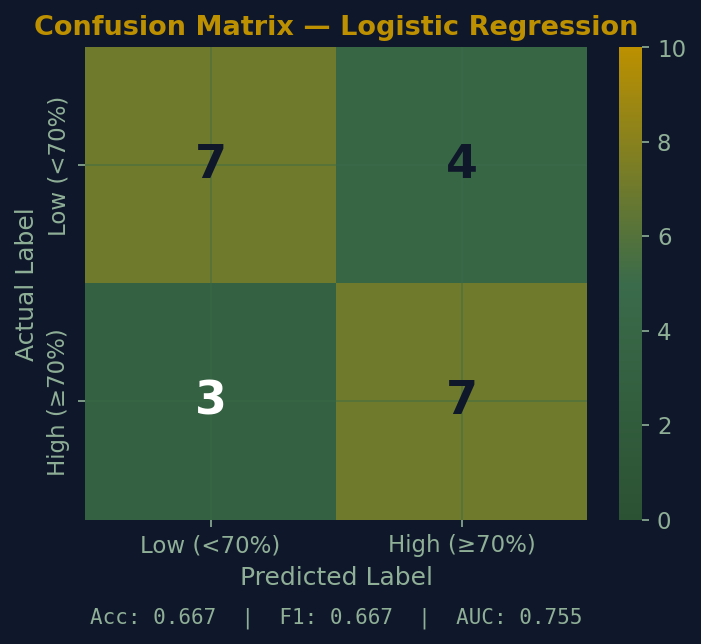
\includegraphics[width=0.35\textwidth]{5feat_behavioral_confusion_Logistic_Regression.png}
    \caption{Confusion matrix for Logistic Regression}
    \label{fig:lr_confusion}
\end{figure}

\begin{figure}[!t]
    \centering
    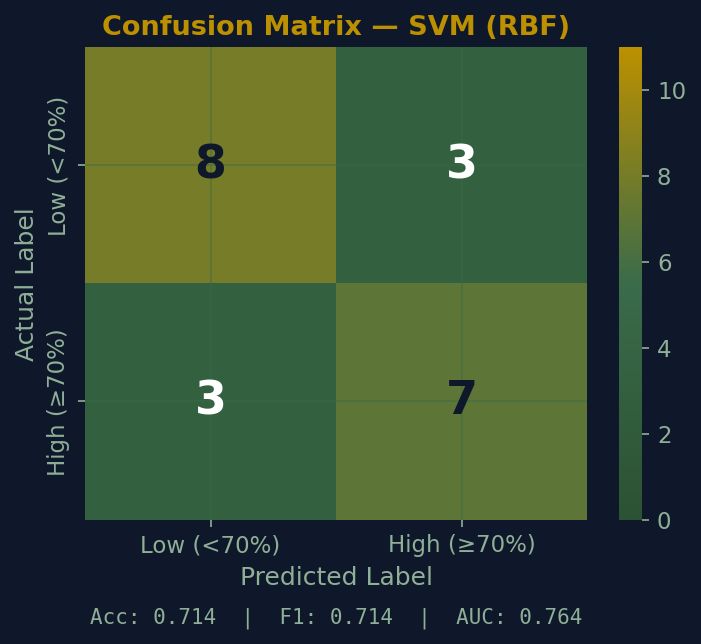
\includegraphics[width=0.75\linewidth]{5feat_behavioral_confusion_SVM_RBF.png}
    \caption{Confusion matrix for SVM (RBF)}
    \label{fig:svm_confusion}
\end{figure}

The confusion matrices highlight distinct differences in model behavior:

\begin{itemize}
    \item \textbf{Logistic Regression} provides a strong linear baseline,
    capturing much of the behavioral signal with relatively balanced
    performance across classes.
    \item \textbf{SVM (RBF)} provides the most stable and accurate
    classification, with strong performance on both classes and
    fewer extreme errors.
\end{itemize}
Errors are concentrated among students near the performance threshold (60–75\%), suggesting that borderline learners exhibit less distinct behavioral patterns. This pattern is consistent with prior EDM findings that borderline learners exhibit mixed or unstable behavioral signatures \cite{baker2009state, romero2010edm}.

Together, these results show that behavioral signals alone can predict student performance, but the signal gets noisier for students near the mastery threshold.

\subsection{ Feature Importance and SHAP Interpretability}

Interpretability analyses were conducted using both model‑based (Random Forest Gini importance) and model‑agnostic (SHAP) methods.
On the full 16‑feature set, difficulty‑weighted features dominate importance rankings, confirming leakage. However, timing and pacing features still contribute meaningfully.

\begin{figure}[!t]
    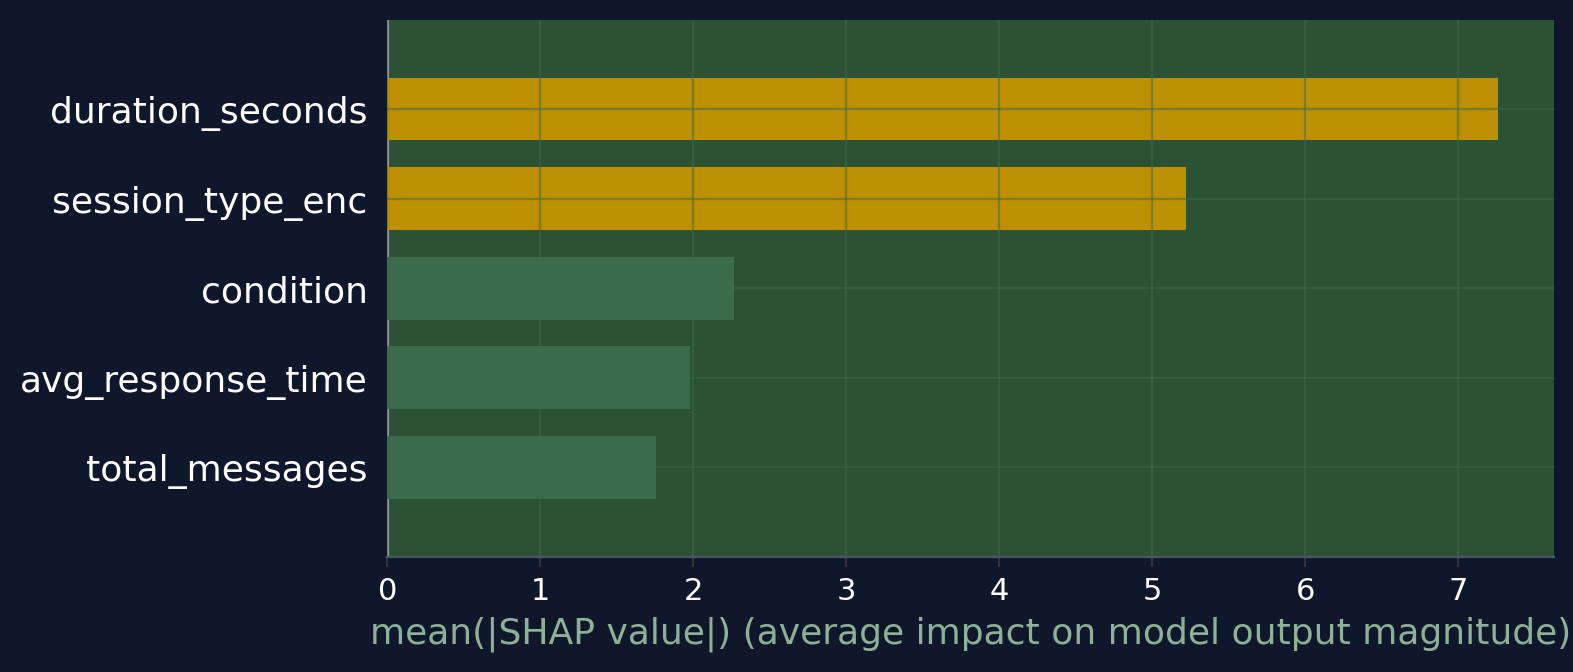
\includegraphics[width=.90\linewidth, height=0.90\textheight, keepaspectratio]{shap_bar_5feat_behavioral.png}
    \caption{SHAP feature importance for the 5-feature model.}
    \label{fig:shap_5feat}
\end{figure}

\begin{figure}[!t]
    \centering
    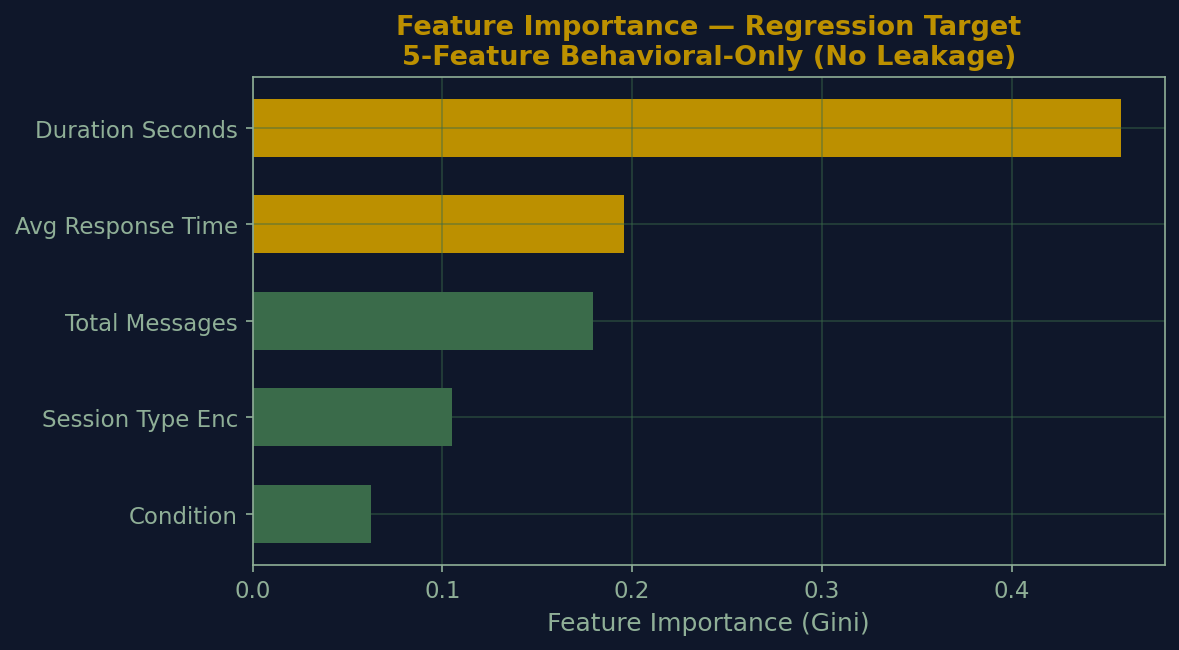
\includegraphics[width=.90\linewidth, height=0.90\textheight, keepaspectratio]{5feat_behavioral_feature_importance.png}
    \label{fig:featureimportance_5feat}
    \caption{Gini feature importance for the 5-feature model.}
\end{figure}

On the refined 5‑feature behavioral model, SHAP reveals a consistent global pattern:
\begin{itemize}
    \item \textbf{duration\_seconds} is the strongest predictor
    \item \textbf{session\_type\_enc} and condition provide structural context
    \item \textbf{avg\_response\_time} captures pacing and cognitive load
    \item \textbf{total\_messages} reflects engagement depth
\end{itemize}

The agreement between Gini importance and SHAP strengthens confidence that these behavioral signals are robust and not artifacts of a single model.

\subsection{Ablation Study}

Table \ref{table:ablation} shows the change in accuracy from the presence and removal of the difficulty features. 
\begin{table}[H]
\centering
\caption{Ablation Study Results}
\begin{tabular}{lcc}
\toprule
Model & CV Before & CV After \\
\midrule
GBM & -0.14 & -0.29 \\
SVM (RBF) & +0.04 & +0.08 \\
\bottomrule
\end{tabular}
\label{table:ablation}
\end{table}

The ablation results highlight how removing difficulty-weighted
features affects model generalization. Gradient Boosting performs
substantially worse after the removal of these features, with
cross-validated accuracy decreasing from $-0.14$ to $-0.29$.
This decline reflects the model’s reliance on difficulty-weighted
signals, which partially encode quiz outcomes and inflate
performance on the full feature set.

In contrast, SVM (RBF) improves under the leakage-free
formulation (from $+0.04$ to $+0.08$), indicating that
difficulty-weighted features introduce noise for models that rely
on smooth, nonlinear decision boundaries. Logistic Regression
shows a similar qualitative improvement in stability, while
Random Forest exhibits moderate sensitivity, becoming more
consistent on the behavioral-only set.

Overall, removing difficulty-weighted features improves
generalization for several models, particularly SVM and
Logistic Regression, confirming that leaked features distort
model behavior and mask the true predictive value of behavioral
signals.

\section{Related Work}


Research in Artificial Intelligence in Education (AIED) spans intelligent
tutoring systems, adaptive feedback, and student modeling
\cite{woolf2013aied}. Early intelligent tutoring systems
(ITS) relied on rule-based and model-tracing architectures to provide
structured scaffolding and individualized support, demonstrating
consistent learning gains in domains such as programming
\cite{koedinger2015learning}. Machine learning has long played a role in
these systems: tutors use ML techniques to infer student knowledge,
identify learning strategies, and adapt instruction based on patterns in
tutor–student interactions \cite{woolf2013aied}. These approaches show that behavioral traces, rather than correctness alone, can serve as meaningful signals for personalization.

Educational Data Mining (EDM) has further established that behavioral
features such as timing, pacing, hesitation, and engagement depth carry
predictive value for student performance \cite{romero2010edm,
baker2009state}. Large-scale studies of internet usage and LMS
clickstream data demonstrate that interaction behaviors can differentiate
performance groups and support early identification of at-risk learners
\cite{xu2019internetusage}. These works highlight that temporal patterns,
connection frequency, and engagement discipline are predictive of
academic outcomes, even without access to correctness-based features.
Recent MOOC research similarly shows that event-level interaction logs
can be used to cluster learners and predict behavioral trajectories with
high accuracy \cite{chonraksuk2024thaiMOOC}. However, these systems
primarily rely on platform-level telemetry rather than fine-grained,
session-level learning interactions.

Clickstream-based predictive modeling has also been applied to early
warning systems. Borna et al. \cite{10.3389/feduc.2024.1421479} found that ML models trained on LMS interaction logs effectively identify at-risk
students, though predicting high achievers remains challenging due to
the complex relationship between engagement patterns and academic
success. This limitation underscores the need for more nuanced
behavioral modeling approaches that move beyond coarse interaction
counts.

Within programming education, prior work has focused on IDE telemetry,
code snapshots, and compilation events as predictors of learning
outcomes \cite{piech2015deep, rivers2017automated}. Far less attention
has been given to conversational interaction logs from AI tutors,
especially those powered by large language models. Existing studies on
LLM-based tutoring primarily evaluate learning gains, usability, or
student perceptions \cite{kasneci2023chatgpt}, rather than treating the
interaction itself as a behavioral dataset for predictive modeling.

This work contributes to the literature by demonstrating that
session-level behavioral features extracted from LLM tutor logs can
predict short-term quiz performance above chance, even without
correctness-based features. It also identifies and corrects a form of
data leakage introduced by difficulty-weighted quiz features, emphasizing
the importance of rigorous feature design when modeling learning
outcomes. To our knowledge, this is one of the first empirical analyses
to use LLM tutor interaction logs from a controlled study as a predictive
modeling dataset in novice programming contexts.


\section{Discussion}

\subsection{Uniqueness and Ethical Considerations}

Many predictive models in education rely on demographic variables, prior academic history, or socio‑economic indicators. While these features often improve accuracy, they risk reinforcing existing inequities by embedding structural biases into algorithmic predictions. Behavioral‑only models offer a more equitable alternative: they rely solely on how a student interacts with the learning environment, not who the student is or what background they come from. By focusing on pacing, duration, and message patterns, this study avoids demographic proxies and instead models the learning process itself. The ablation study confirms that these behavioral features are sufficient to predict performance above chance, even when correctness‑adjacent features are removed. This approach aligns with emerging ethical guidelines in AIED, emphasizing fairness, transparency, and the minimization of bias in algorithmic decision‑making.

This study reframes AI tutoring interactions as a real-time behavioral dataset suitable for predictive modeling. Unlike traditional approaches that rely on post-hoc metrics, interaction logs provide continuous signals that can support early intervention.

The results demonstrate that behavioral features—pacing, duration, and interaction structure—are sufficient to predict performance above chance. These features are also inherently actionable: an AI tutor can detect rapid responses or shallow engagement and adapt instruction accordingly.

 Finally, the identification of leakage underscores the importance of careful feature design. Without proper validation, models may appear highly accurate while relying on invalid signals.

\subsection{Practical Implications for Adaptive Learning}

This study demonstrates that interaction-log features provide a non-intrusive, real-time mechanism for diagnostic assessment. By prioritizing behavioral signals over performance-based metrics, tutoring systems can mitigate the risks of data leakage and provide pedagogical interventions—such as adjusting scaffolding depth or triggering metacognitive prompts—well before a student reaches the final assessment phase. These results position the AI tutor not as a static instructional tool, but as a sensitive diagnostic engine capable of flagging behavioral patterns associated with cognitive struggle.

\section{Conclusion}

\subsection {The Impact of Feature Refinement and Leakage Removal}

Initial modeling on the full 16-feature set yielded performance metrics that, while seemingly strong, were identified as being artificially inflated by data leakage. Feature importance analysis revealed that difficulty-weighted metrics, derived from quiz responses, partially encoded the target variable. This realization necessitated a pivot to a more rigorous analytical narrative focused exclusively on session-level behavioral signals.

\subsection{Interpretability and Behavioral Signals}

The convergence of SHAP values and Gini importance confirms that session duration, message pacing (average response time), and engagement depth (total messages) are the most robust indicators of short-term mastery. On the leakage-free behavioral formulation, the Support Vector Machine with an RBF kernel achieved the strongest and most stable performance (test accuracy = \textbf{0.714}, 5‑fold CV = \textbf{0.681}, AUC‑ROC = \textbf{0.764}), indicating the strength of behavioral signals and demonstrating that AI tutoring systems can identify at‑risk students in real time based on conversational cadence.



\bibliographystyle{IEEEtran}
\bibliography{references}

\end{document}
